\documentclass[12pt,a4paper]{article}
\usepackage[utf8]{inputenc}
\usepackage[T1]{fontenc}
\usepackage{ucs}
\usepackage{amsmath}
\usepackage{amsfonts}
\usepackage{amssymb}
\usepackage{amsthm}
\usepackage{mathtools}
\usepackage[english]{babel}
\usepackage{svg}	
\usepackage{graphicx}
\usepackage{cite}
\usepackage{url}
\usepackage{color}
\usepackage{smartdiagram}
\usepackage{subfig}
\usepackage{booktabs}

\author{Martí Municoy, Alba Gordó, Jan-Hendrik Niemann\\ and Andreas Radke}
\title{Research and Innovation}

%\begin{filecontents*}{geojson.csv}
%City;Geojson Source
%Berlin;https://github.com/m-hoerz/berlin-shapes
%Barcelona;https://github.com/martgnz/bcn-geodata/find/master
%Hamburg;https://matthiassuessen1975.carto.com/tables/bezirke\_in\_hamburg/public/map
%München;https://mucx.carto.com/tables/osm\_muc\_bezirke/public
%Paris;https://github.com/blackmad/neighborhoods/blob/master/gn-paris.geojson
%New York;https://github.com/blackmad/neighborhoods/blob/master/new-york-city-boroughs.geojson
%London;https://joshuaboyd1.carto.com/tables/london\_boroughs\_proper/public
%Madrid;https://github.com/codeforamerica/click\_that\_hood/blob/master/public/data/madrid-districts.geojson
%Sydney;http://insideairbnb.com/get-the-data.html
%Brussels;http://insideairbnb.com/get-the-data.html
%Hong Kong;http://insideairbnb.com/get-the-data.html
%Vancouver;http://insideairbnb.com/get-the-data.html
%San Francisco;http://insideairbnb.com/get-the-data.html
%Palo Alto;http://insideairbnb.com/get-the-data.html
%Chicago;http://insideairbnb.com/get-the-data.html
%Los Angeles;http://insideairbnb.com/get-the-data.html
%\end{filecontents*}

\begin{document}
	\maketitle
	
\subsection*{Abstract}

\textcolor{red}{TODO: modify the abstract s.t. it fits to the content}
The aim of this project is to find and visualize the events posted on Meetup.com in different cities in order to analyze the density of planned activities and to make a social study regarding typical meeting times and most usual activities and interests. One aspect may concern different meeting times in Spain and Germany or group size. We will focus our research on cultural activities like languages tandems and sports. The data shall be obtained via the Meetup-API and OpenStreetMap. The most important data source for this project is the Meetup-API where we have to request the events with different Python packages like “requests” or “meetup-api”. Our second task is to visualize the locations of the events on a given city map obtained by data resources like OpenStreetMap. To plot the locations we could use “matplotlib” or similar Python plotting libraries.
One further aspect could be to look for interest of twitter users to make recommends to activities nearby. The geotag of the tweets provides the central information for the search.

\tableofcontents
	
\section{Summary and Goals}\label{sec:summaryandgoals}

The human being is social. Every day there are millions of events. Thousands of them are posted at the webpage \url{Meetup.com}. It is a website where people can seek and find other people with the same interest. It helps to organize events and makes them public.

This is the reason why we chose \url{Meetup.com} to analyze the behavior and the preferences of cities and its inhabitants all over the world. Almost all \url{Meetup.com} activities contain information about their location, expressed in terms of latitude and longitude. Thus, by using the \url{Meetup.com} API, we can request and extract a dataset "latitude-longitude" for all the available \url{Meetup.com} events. Then, we can use this dataset to plot all these located activities on a \url{GoogleMaps.com} map. Our aim, here, is to create and visualize a density map, a so-called heatmap, where one can see all the activities for a selected city.

Furthermore, \url{Meetup.com} API allows the user to get activities arranged by category. We want to use this tool to consider separately different types of events like "Food \& Drink" or "Sports" and study their relative predominance in different cities. By combining this information with the geographical and/or political structure of a city, one may can also identify trending districts and neighborhoods in a city. To do so we make use of GeoJSON-files which can contain the polygonal shape of a district and its name. There are several websites where one can get GeoJSON data or create his own data. By using the information from these websites, a GeoJSON dataset is created with all the coordinates of the districts for all the studied cities. This constitutes the third data source that is used in this work.

A fourth data source is \url{Wikipedia.org} where a web scraping script is applied on to extract some useful population data such as the population number, the population density or the land area of each district. With all this information, one can use the following factor to evaluate the social activity per district. This factor is given as

\begin{align*}
	\text{Social activity} = \frac{\text{\# events}}{\text{\# person}}.
\end{align*}

Once downloaded, we can access to our data off-line. This is due to the fact that we store it locally by using csv (comma-separated files).

This report is structured as follows in \ref{sec:limitationsandfuturework} sections. Firstly, in section \ref{sec:datalifecycle} we discuss the data life-cycle of our data. In section  \ref{sec:toolsanddata}, we present both, the third-party tools that we used and the custom methods that we developed in our own, to achieve this project. They mainly, are developed by using Python.  Afterwards, we present our results in section \ref{sec:results} and, in section \ref{sec:legalandethicalissues}, we make a legal and ethical disquisition. Finally, in section \ref{sec:limitationsandfuturework} we discuss the limitations of our work and make proposals for future work.
\section{Data Life Cycle}\label{sec:datalifecycle}

%\smartdiagram[circular diagram:clockwise]{Creation, Storage, Use, Sharing, Archiving, Destruction}

In the following section we have a closer look at the terms \emph{data life cycle} and \emph{data life cycle management}.

\emph{Data life cycle} is a term which tries to describe the life of data and information. Since there is no unique definition of a data life cycle, we define the folloing six stages: creation, storage, use, sharing, archiving and destruction  \cite{marburg}, \cite{spirion}.

\begin{enumerate}
	\item \textbf{Creation}: Data is created. It can be created as a structured or unstructured set of data, can be obtained by collection, measurements, generated or gathered. We create our data by using the Meetup-API. By performing a web scraping at \url{Wikipedia.org} we gather the number of population, the population density and the land area for different cities and their districts. In this way, we request and create the data which is going to be needed for this project.
	\item \textbf{Storage}: Once the data is created, it has to be stored. Depending on where we want to apply this data for, there are different and optimal kinds of storage solutions. However, this is not subject of this report. In our case, both, the data gathered from \url{Meetup.com} and \url{Wikipedia.org}, are saved as csv-files on the hard drive. As a version control system we used Git and additionally stored our data on \url{github.com} for better collaboration.
	\item \textbf{Use}: Data can be viewed, modified, analyzed, corrected, interpreted, visualized and joined. We use our data to visualize the social activity of cities. We join our data from different sources and visualize it on a given map which can be seen as data as well. This data visualization and its further treatment can be used to obtain new data such as the measurement of the social activity per district introduced in section \ref{sec:summaryandgoals}.
	\item \textbf{Sharing}: Data can be shared. There are several ways of sharing by using different file formats, applications or operating environments. In this work, we used csv-files and GeoJSON-files to share data from one method to another. For instance, the district coordinates are read from a GeoJSON-file, the Meetup events and the population data from a csv-file. Then, these are the files created by the scripts to share data along different methods.
	\item \textbf{Archiving}: When the data leaves the active use, one should archive it in a suitable way. Since archiving is very similar to storaging, one can use the same methods. One difference may be that saved data needs to be compressed to save storage or protected to prevent unwanted changed. Therefore, the access is slightly more difficult than for data in active use. The file formats used in this project does not satisfy this statement. This is due to the fact that the file formats are chosen to ease the access to their data rather than to save storage space. If we want to keep this data for a long time, we should think on developing a method to compress this data.
	\item \textbf{Destruction}: There is a last stage in the data life cycle. There are several reasons why one should destroy data. On one hand, the volume of archived data increases and one needs to save storage to store new data. On the other hand, data gets old and could be not needed anymore. Or, if it is not up to date, it can be replaced by newer versions. The second case is applicable for our work. During every single run of the program new csv-files with event data and new csv-files containing populations data are created. Especially the event data underlie a rapid change.
\end{enumerate}

The term \emph{data life cycle management} describes the process that helps to organize the flow of data throughout its life cycle.
\section{Data Tools}\label{sec:toolsanddata}
\subsection*{Python Packages} 
The main work for our project is done in the Python programming language in version 3.6 \cite{python}. This programming language is used to develop different packages. Each package is in charge of managing a specific dataset and it does a certain job. In this section, we are going to introduce the most important packages that we have developed and used to retrieve the data of this project.

\subsection*{Meetup Package}
This package has the main purpose of retrieve the information of all the available events in a city. Its main module is called \textit{mu\_requests.py}. This module makes use of the \textit{Python 3.6 Requests} package \cite{requests} to submit queries to the Meetup API \cite{meetupapi}. It is able to get information about all the available categories and events. Then, it can also parse the data coming from the Meetup client, whose format is expressed in JSON, and it can store it in a local drive by writing a custom csv file. For instance, all the events found in a city they are written in this way \textit{./csv/name\_of\_the\_city.csv}. This custom csv-file contains all the events of a city arranged by category.

\subsection*{Mapping Package}
This is the package responsible of plotting all the located events on a map. To do this, first, it needs to read all the events data from the previous csv-file. Then, it uses the read coordinates to display events on a \emph{Google Maps} map. This functionality uses the \textit{gmaps} library \cite{gmaps} along with a \textit{Jupyter notebook} \cite{jupyter} which allow us to display data on a map.

It has some tools that allows us manage which events we want to display. For example it allows us to plot only those events that are scheduled in a certain time range or those events which belong to a specific category. We can also control the way the script colors the event marks or their opacity.

Another interesting tool that this package offers is to plot the districts of a city. In this case, \emph{GeoJSON}-files with the delimiting points for each district are required. If you want to plot them according to their population, population data for each district is also required. The script reads these files, parses the data and it can plot and paint the districts according to the number of events per capita that each district has.

\subsection*{Scraping Package}
This package is involved on retrieving data from \url{Wikipedia.org}. Particularly, it searches for the pages belonging to the districts of a city to retrieve information about their population from one of their tables. This process is known as web scraping. To check for the appropriate tables, it uses \textit{BeautifulSoup} Package that is an \emph{HTML} parser.

Then, the script is designed to look for these tables in an intelligent way.  So it is able to check different Wikipedia addresses to get the right information.  Firstly, it looks for the English articles but, in some cases, best articles are written in other languages rather than English. So it is also able to check pages written in Spanish and German.

Once it gets the right population table it comes to the hardest part. It needs to move around the table to look for the proper cells. The functions that are used in the parsing process are able to work with tables, words and numbers expressed in different formats. For instance it supports tables with joined cells or which arrange their information in different ways.

\subsection*{Plotting Package}
The last developed Package is used to plot data from all these retrieved events. It is useful to view and compare the amount of events for each category or city. This script makes use of \textit{pygal package} \cite{pygal} to create mostly bar charts. 

\subsection*{Data}

As already noted we used the data sources that are summarized below:

\begin{itemize}
\item Meetup API: To get the events in the examined cities. 
\item Wikipedia: For obtaining data about the population density of the cities and their districts. 
\item GeoJSON Files: To visualize districts onto Google Maps. Files are obtained from various resources. For the detailed sources see Appendix \ref{subsec:geojson}.
\item Google Maps: As a general back-end for our visualization \cite{googlemaps}.
\end{itemize}
\section{Results}\label{sec:results}

To draw meaningful conclusions we created several types of visualization of the data. First and foremost we plotted the open events onto a map - either as a point map, e.g Figure \ref{fig:barcelonapoints}, or as a occurrences distribution map for each city district, e.g. Figure \ref{fig:barcelonamap}. Additionally numerous bar charts were created with the number of categories (absolute and per capita) per city, compare Figure \ref{fig:barcelonabar}, and vice versa. 

In this chapter we will shortly discuss several cities and their interesting characteristics. 

\begin{figure}[!htp]
	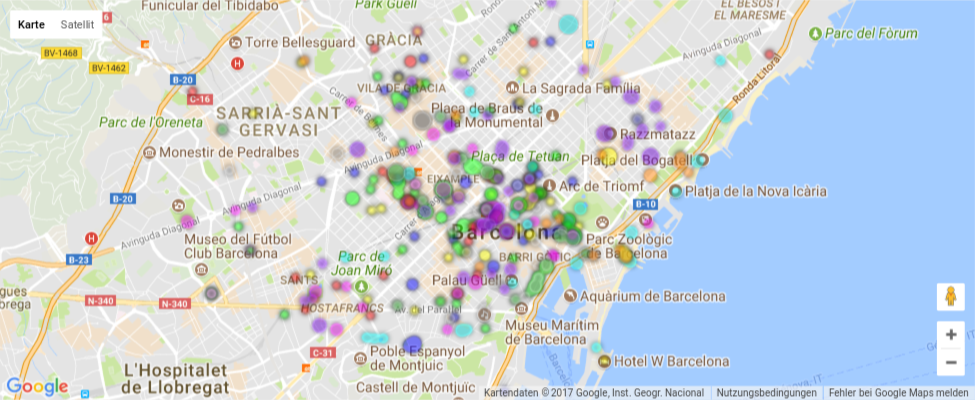
\includegraphics[width=1\linewidth]{images/Barcelona_points.png}
	\caption{Snippet of Barcelona with Open Events}\label{fig:barcelonapoints}	
\end{figure}

\begin{figure}[!htp]
	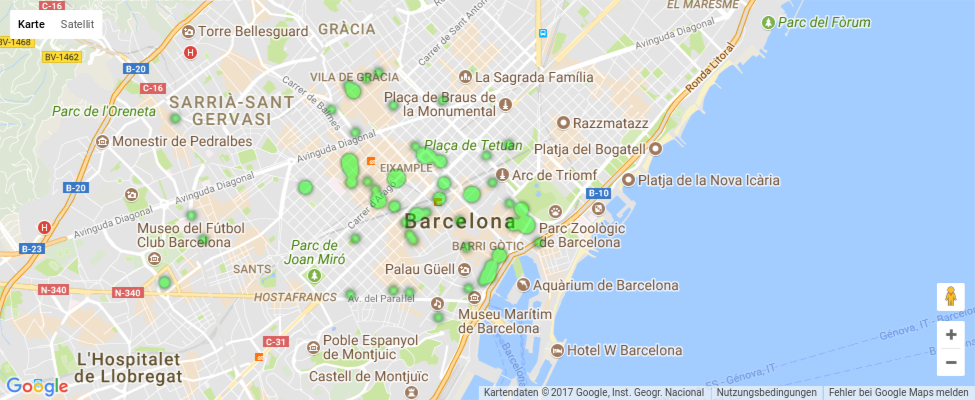
\includegraphics[width=1\linewidth]{images/Barcelona_points_Language.png}
	\caption{Snippet of Barcelona with only Language \& Ethnic Identity Events}\label{fig:barcelonapointslanguage}	
\end{figure}

\begin{figure}[!htp]
	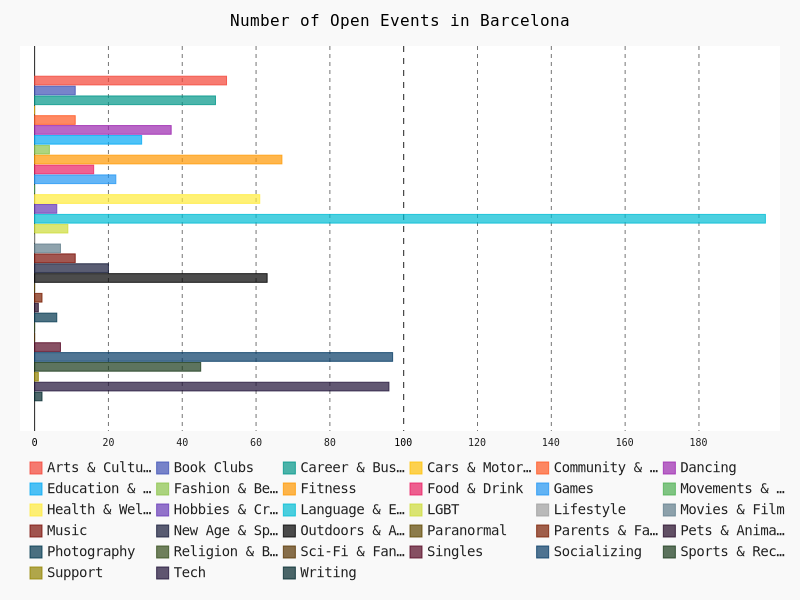
\includegraphics[width=1\linewidth]{../plotting/pngs/categories/Barcelona.png}
	\caption{Activities per Category in Barcelona}\label{fig:barcelonabar}	
\end{figure}

\subsection*{Barcelona}

In Figure \ref{fig:barcelonapoints} one can see an example of Barcelona with open events plotted as points. The different colors represent different Meetup categories. One can see that there are slightly more green points which represent the Meetup category \emph{Language and Ethnic Identity}. A more specific view offers Figure \ref{fig:barcelonapointslanguage} with only the points corresponding to this specific category. Furthermore the already mentioned Chart \ref{fig:barcelonabar} shows that the Language and Ethnic Identity events are indeed the most frequent category which may be an indicator for the diverse and multi-cultural Catalan capital. 

\begin{figure}[!htp]
	% Maximum length
	\subfloat[Activity per District]{\label{fig1:a}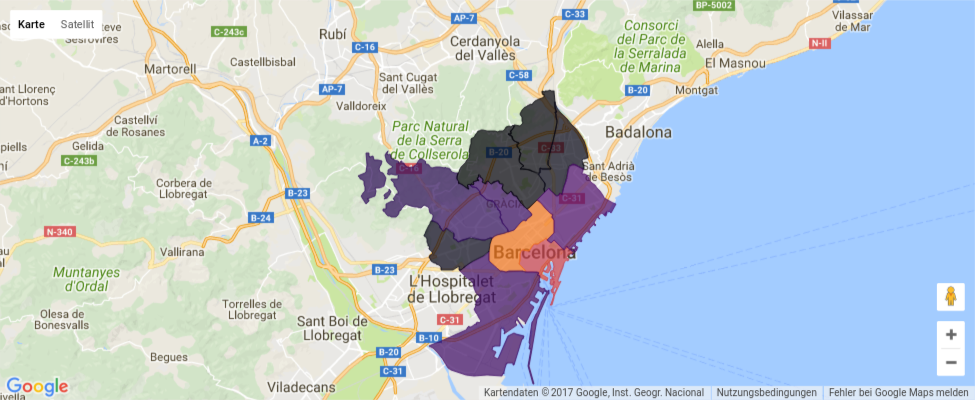
\includegraphics[width=0.49\linewidth]{images/activities_of_districts/Barcelona.png}}\hfill
	\subfloat[Activity per Capita per District]{\label{fig1:b}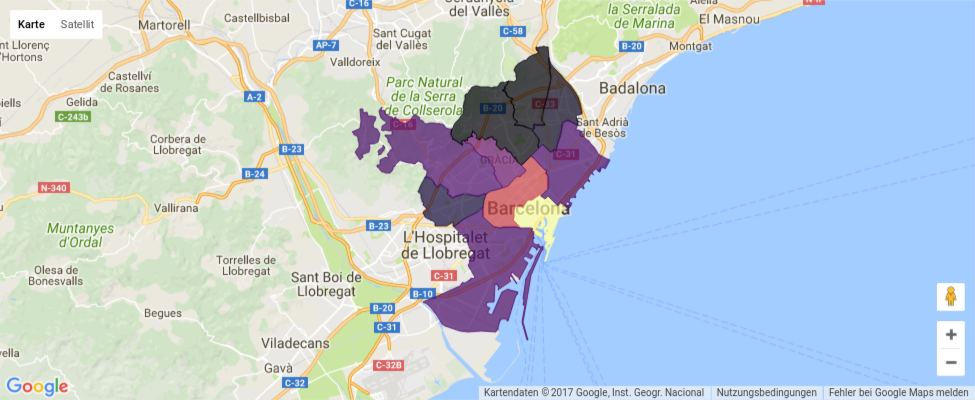
\includegraphics[width=0.49\linewidth]{images/activities_per_capita_of_districts/Barcelona.png}}%
	\caption{Barcelona}\label{fig:barcelonamap}
\end{figure}

The most activities are unsurprisingly in the populous Eixample district but per inhabitant there are more events in Ciutat Vella. Despite having a natural concentration in more centric areas for Barcelona it seems that the activities are a bit more spread out to the whole city. This can be due to Barcelonas small size and its high population density. 
In contrast there are Marid-Centro (Figure \ref{fig:madridmap}), New York-Manhattan (\ref{fig:newyorkmap}) and Hong Kong (\ref{fig:hongkongmap}) where the open events are strongly concentrated in one or a few central districts. 

\subsection*{London}

London seems rather centric with Westminster as the hot-spot district. But especially per capita everything is overshadowed by the small and little populated City of London. Later we will see that London has the highest number of events outside of Europe (in our dataset). 

The most popular categories are Socializing and Tech. 

\begin{figure}[!htp]
	% Maximum length
	\subfloat[Activity per District]{\label{fig1:a}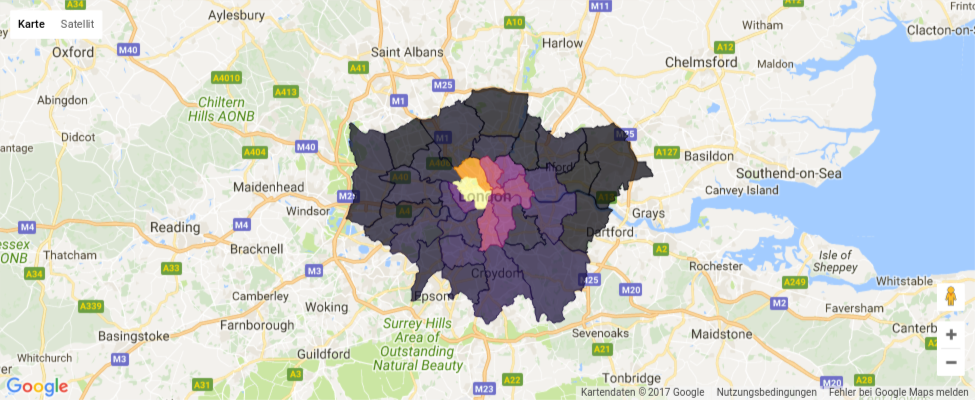
\includegraphics[width=0.49\linewidth]{images/activities_of_districts/London.png}}\hfill
	\subfloat[Activity per Capita per District]{\label{fig1:b}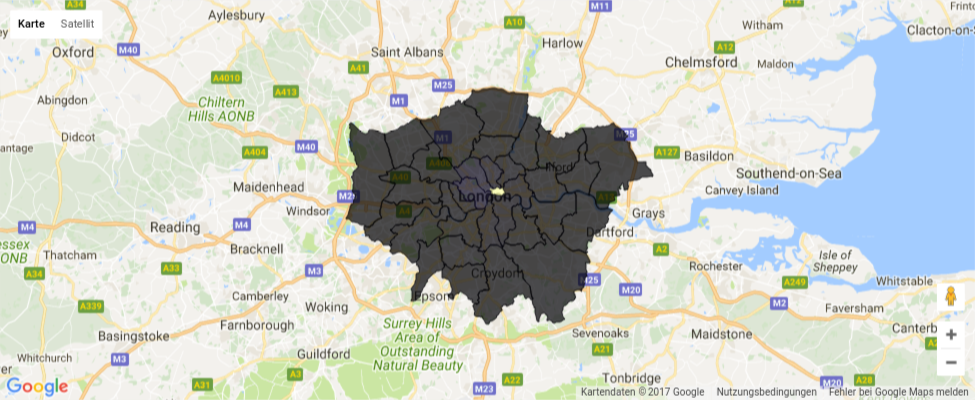
\includegraphics[width=0.49\linewidth]{images/activities_per_capita_of_districts/London.png}}%
	\caption{London}
\end{figure}


\subsection*{Berlin}

Because of the historical division of Berlin it does not have one big city center. One can see (Figure \ref{fig:berlinpoints}) that event concentration is slightly shifted to the east around Prenzlauer Berg (south of Pankow, East of Mitte and Friedrichshain-Kreuzberg. In contrast there is only a smaller focus at the City West (Zoologischer Garten, Charlottenburg-Wilmersdorf). 

\begin{figure}[!htp]
	% Maximum length
	\subfloat[Activity per District]{\label{fig1:a}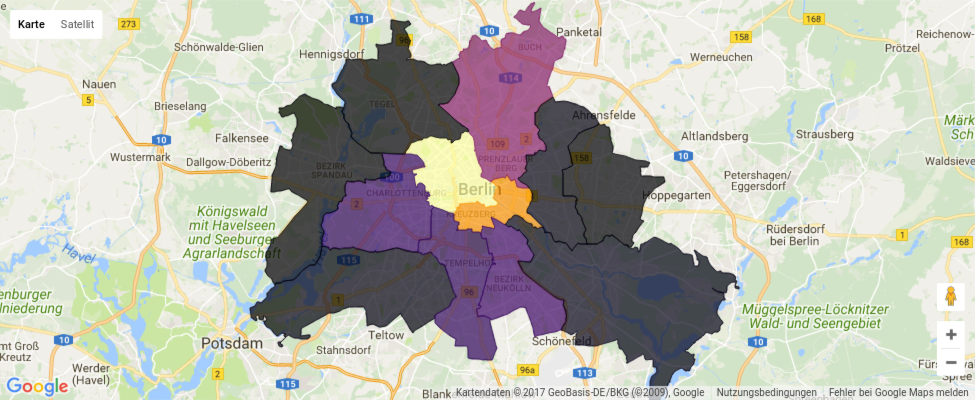
\includegraphics[width=0.49\linewidth]{images/activities_of_districts/Berlin.png}}\hfill
	\subfloat[Activity per Capita per District]{\label{fig1:b}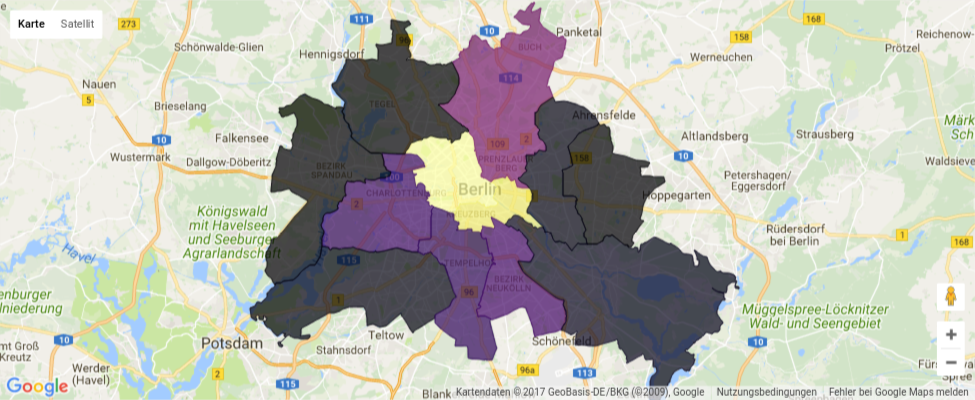
\includegraphics[width=0.49\linewidth]{images/activities_per_capita_of_districts/Berlin.png}}%
	\caption{Berlin}
\end{figure}


\begin{figure}[!htp]
	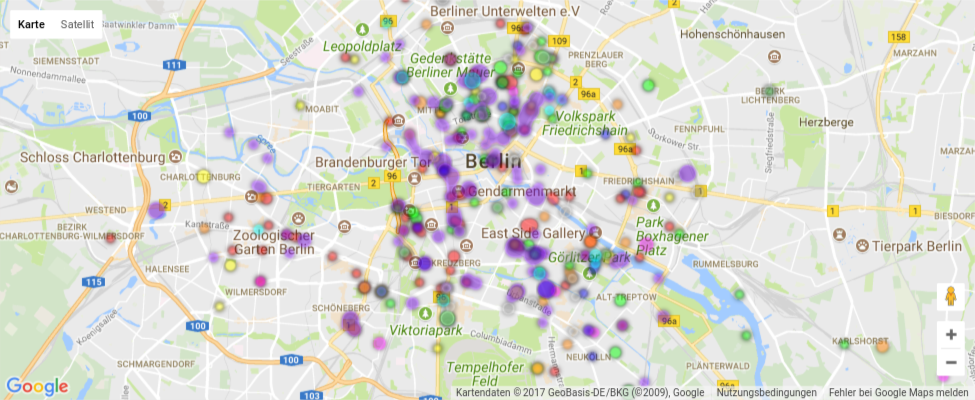
\includegraphics[width=1\linewidth]{images/Berlin_points.png}
	\caption{Snippet of Berlin with Open Events}\label{fig:berlinpoints}	
\end{figure}

Regarding the categories (\ref{fig:berlinbar}) it is obvious that the \emph{Tech} activities dominate in Berlin. The reason for this increased interest in technology may be due to a high number of upcoming startups. 
But actually the high dominance (three times larger than the second favorite; largest dominance) of technology events in contrast to other categories is a trait which all three examined German cities share. One conclusion would that Meetup seems so far to be limited to \emph{tech-interested} people in Germany. 

\begin{figure}[!htp]
	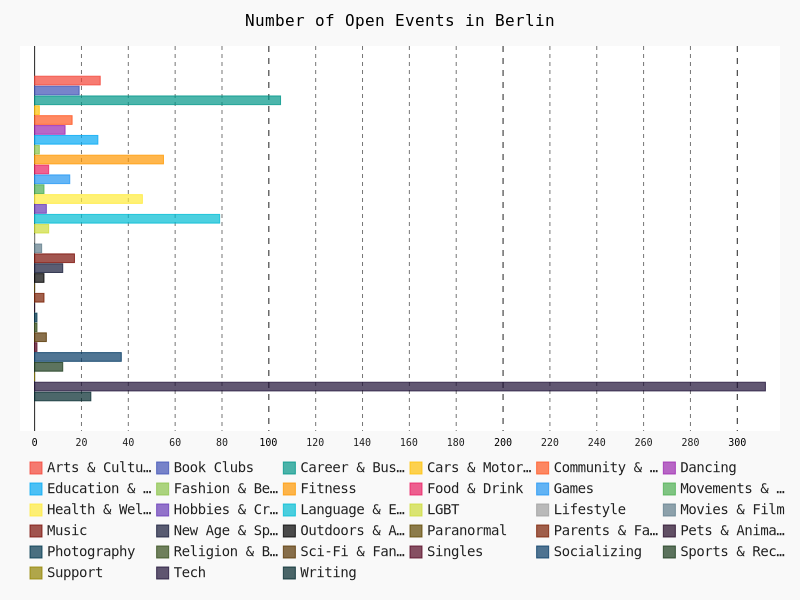
\includegraphics[width=1\linewidth]{../plotting/pngs/categories/Berlin.png}
	\caption{Activities per Category in Berlin}\label{fig:berlinbar}	
\end{figure}


\subsection*{Madrid}

Almost all events are concentrated in Madrid-Centro. Madrid's most favorite categories are by far Tech and Languages \& Ethnic Identity. 

\begin{figure}[!htp]
	% Maximum length
	\subfloat[Activity per District]{\label{fig1:a}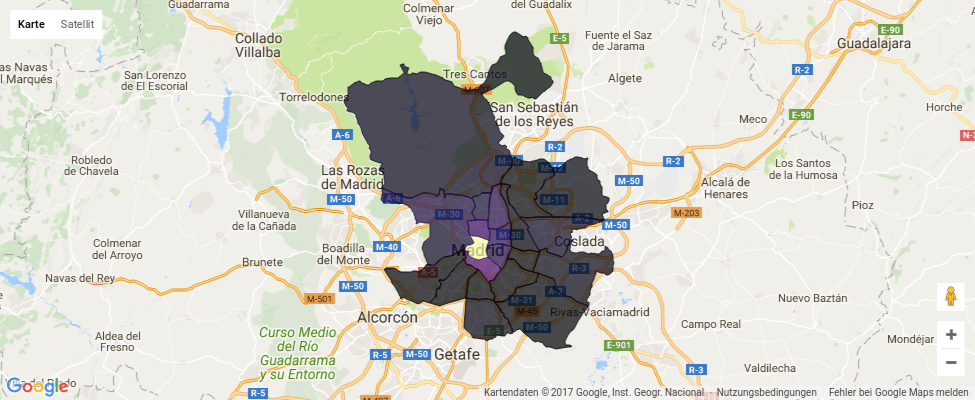
\includegraphics[width=0.49\linewidth]{images/activities_of_districts/Madrid.png}}\hfill
	\subfloat[Activity per Capita per District]{\label{fig1:b}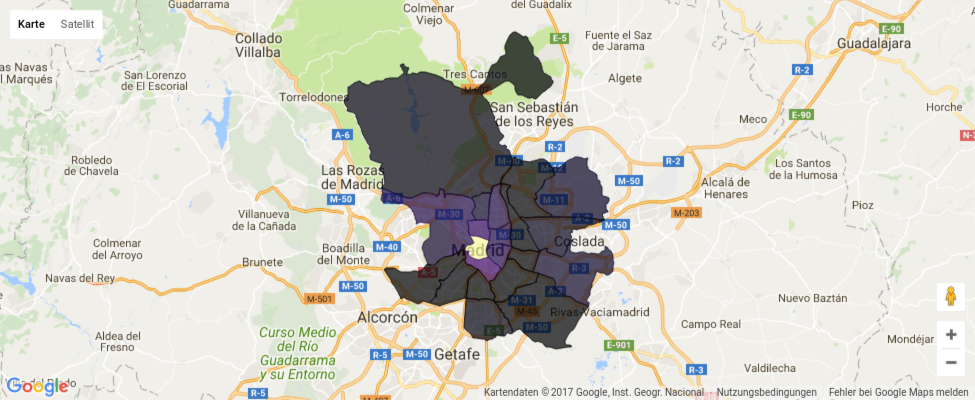
\includegraphics[width=0.49\linewidth]{images/activities_per_capita_of_districts/Madrid.png}}%
	\caption{Madrid}
\end{figure}

\subsection*{Paris}

Paris is an example for a more evenly distributed city - at least in the total number of events per district. This may be due to its small size and dense population (compare Barcelona). The picture would probably be different if one considers the vast metropolitan area of Paris with its 12 Mio. people and its area of 17000 $ km^2 $ (in contrast to the actual 2.2 Mio. and 105 $ km^2 $)
Again Tech and Language and Ethnic Identity are the most favored categories. 

\begin{figure}[!htp]
	% Maximum length
	\subfloat[Activity per District]{\label{fig1:a}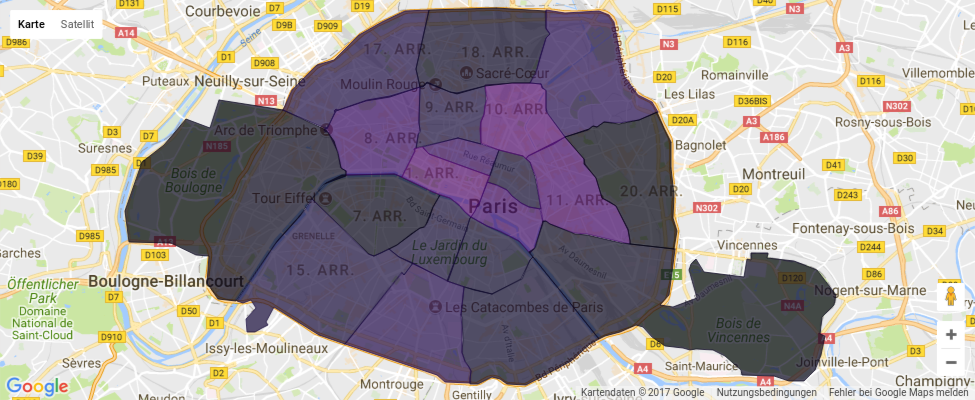
\includegraphics[width=0.49\linewidth]{images/activities_of_districts/Paris.png}}\hfill
	\subfloat[Activity per Capita per District]{\label{fig1:b}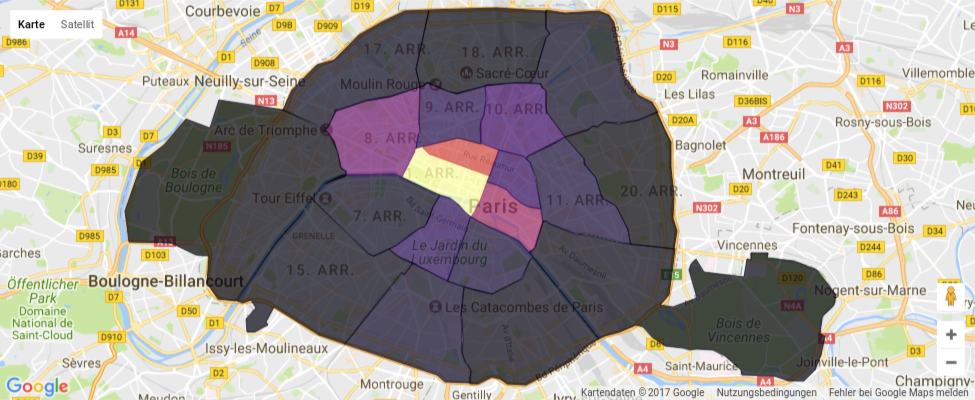
\includegraphics[width=0.49\linewidth]{images/activities_per_capita_of_districts/Paris.png}}%
	\caption{Paris}
\end{figure}


\subsection*{Brussels}

In this case we actually did not consider the City of Brussels but rather the Brussels-Capital Region. But one can clearly see the bright yellow shape which represents the City of Brussels (this is one \emph{district}!). Per capita some central regions like Ixelles show a higher activity too. 
\begin{figure}[!htp]
	% Maximum length
	\subfloat[Activity per District]{\label{fig1:a}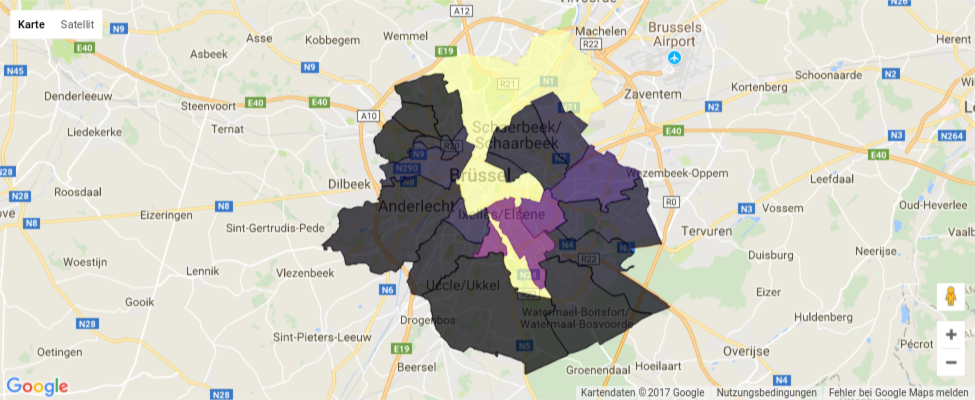
\includegraphics[width=0.49\linewidth]{images/activities_of_districts/Brussels.png}}\hfill
	\subfloat[Activity per Capita per District]{\label{fig1:b}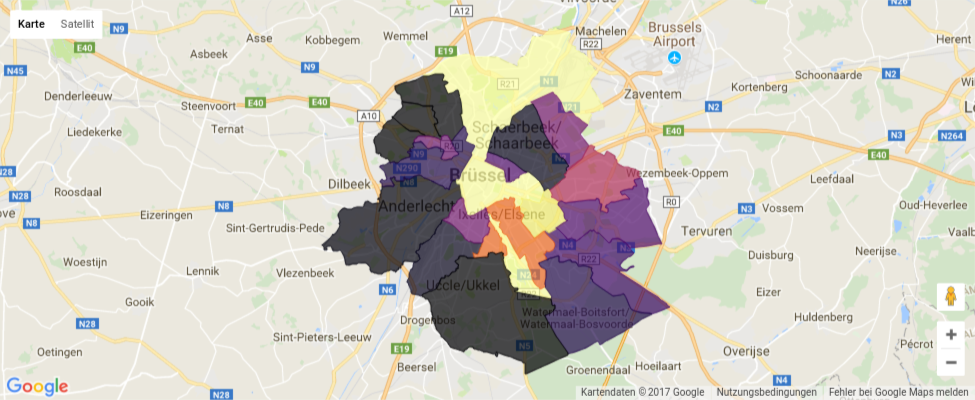
\includegraphics[width=0.49\linewidth]{images/activities_per_capita_of_districts/Brussels.png}}%
	\caption{Brussels}\label{fig:madridmap}
\end{figure}

\subsection*{Hamburg}

\begin{figure}[!htp]
	% Maximum length
	\subfloat[Activity per District]{\label{fig1:a}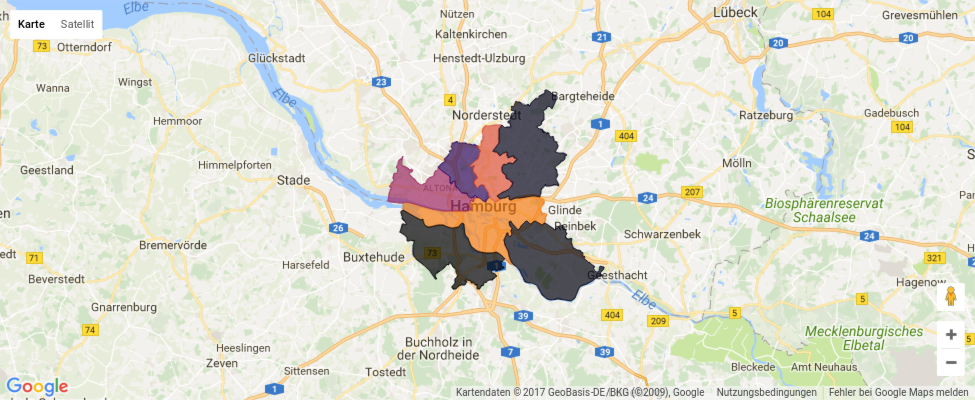
\includegraphics[width=0.49\linewidth]{images/activities_of_districts/Hamburg.png}}\hfill
	\subfloat[Activity per Capita per District]{\label{fig1:b}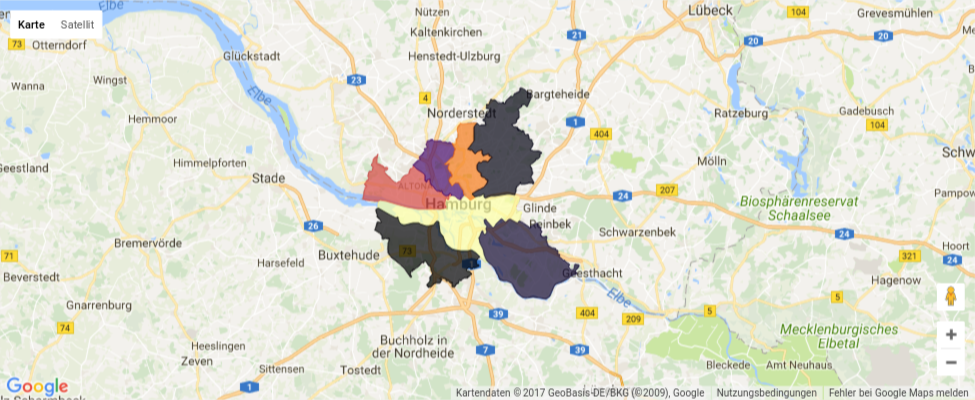
\includegraphics[width=0.49\linewidth]{images/activities_per_capita_of_districts/Hamburg.png}}%
	\caption{Hamburg}
\end{figure}

\subsection*{New York City}

\begin{figure}[!htp]
	% Maximum length
	\subfloat[Activity per District]{\label{fig1:a}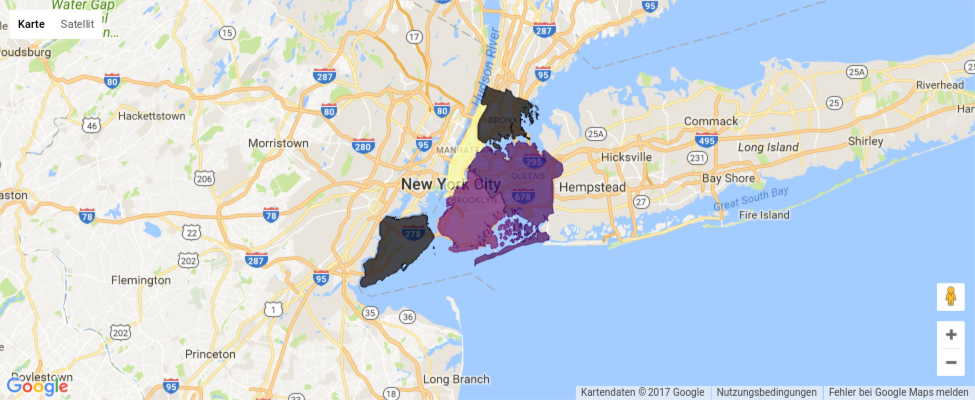
\includegraphics[width=0.49\linewidth]{images/activities_of_districts/NewYork.png}}\hfill
	\subfloat[Activity per Capita per District]{\label{fig1:b}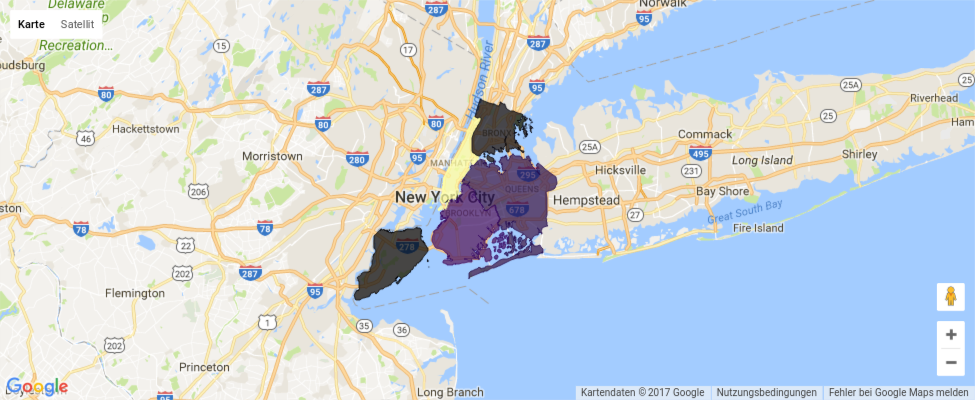
\includegraphics[width=0.49\linewidth]{images/activities_per_capita_of_districts/NewYork.png}}%
	\caption{New York City}\label{fig:newyorkmap}
\end{figure}

\subsection*{Munich}

\begin{figure}[!htp]
	% Maximum length
	\subfloat[Activity per District]{\label{fig1:a}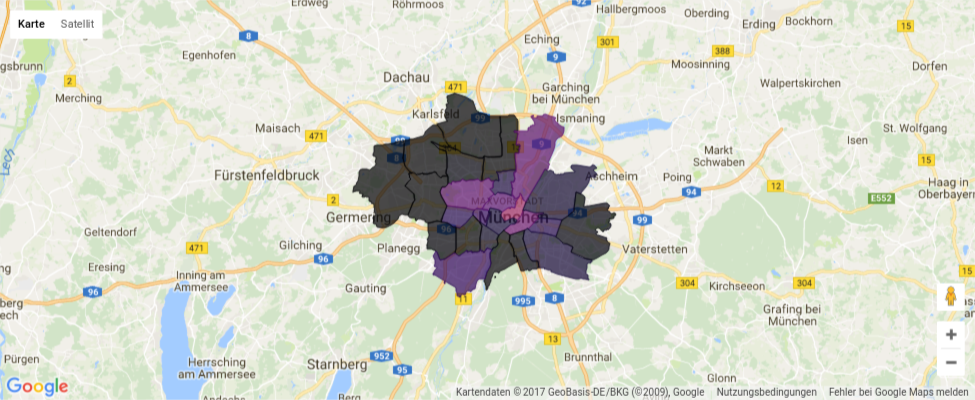
\includegraphics[width=0.49\linewidth]{images/activities_of_districts/Munich.png}}\hfill
	\subfloat[Activity per Capita per District]{\label{fig1:b}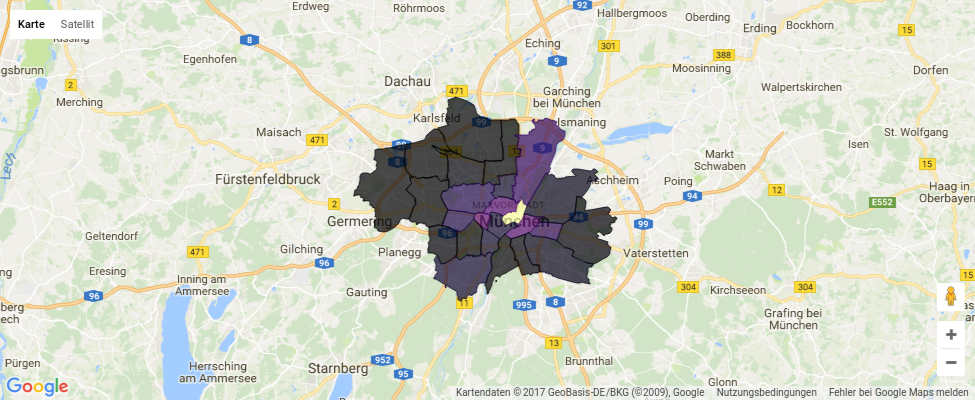
\includegraphics[width=0.49\linewidth]{images/activities_per_capita_of_districts/Munich.png}}%
	\caption{Munich}
\end{figure}

\subsection*{Hong Kong}

\begin{figure}[!htp]
	% Maximum length
	\subfloat[Activity per District]{\label{fig1:a}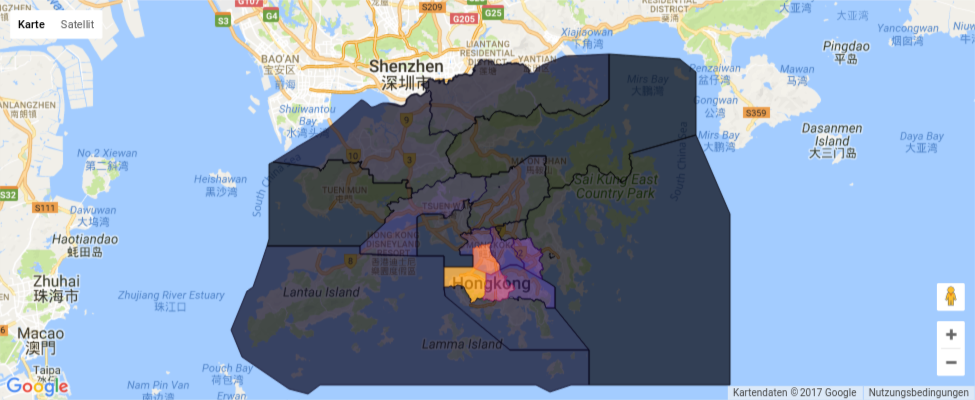
\includegraphics[width=0.49\linewidth]{images/activities_of_districts/HongKong.png}}\hfill
	\subfloat[Activity per Capita per District]{\label{fig1:b}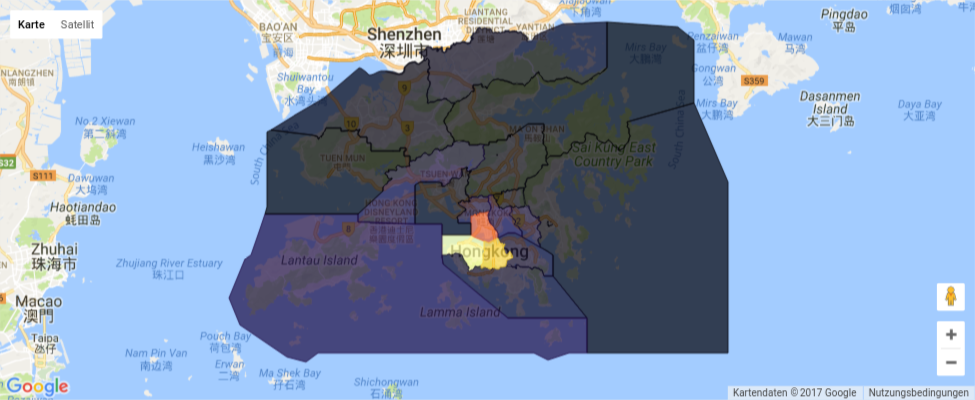
\includegraphics[width=0.49\linewidth]{images/activities_per_capita_of_districts/HongKong.png}}%
	\caption{Hong Kong}\label{fig:hongkongmap}
\end{figure}
\section{Legal and Ethical Issues}\label{sec:legalandethicalissues}
\section{Limitations and Future Work}\label{sec:limitationsandfuturework}

One major issue is that this project is depending strongly on the quality of the data available at \url{Meetup.com}. We have to rely on the users of \url{Meetup.com} so this issue can hardly be improved. One idea would be to integrate other social services like \url{Facebook.com} to extrend our data source and to get more independent. In this way one could also fix the problem that \url{Meetup.com} might be less known in non-English speaking countries. Having a wide base as data source one gets more independent of local and regional preferences regarding the social networks.\\Another problem is that this project has the potential to be extended in the following way: So far our program is restricted to predefined cities. It is not possible to select new cities or regions. This is due to the fact that we work with GeoJSON-files which are saved locally on the hard drive. \textcolor{red}{The second problem is that some Wikipedia pages for the cities are not coherent so that one needs to be careful}. One improvement could be to create a user interface and the possibility to select new cities and regions. By selecting single categories of events one could get special information, e.g. where to go running. Additional, in an application, one could automatically create suitable graphics, charts and tables.\\Another limitation is as well related to \url{Meetup.com}. Seince we only have one data source for events, we only can give sufficient criterions for districts. A district having lots of events seems to be trening. However, a district having less events is not automatically less interesting and popular. It just means that its inhabitants are not using \url{Meetup.com}. Again, one should take more data sources into account.

Our tool could help social scientists to provide theire hypothesis with proving data. Beside literature, studies and surveys our tool seems to be a good method for analyzing the behaviour and preferences of populations.

\section*{Appendix}\label{sec:appendix}

\subsection*{Sources of GeoJSON Files}\label{subsec:geojson}
\begin{table}[h]
	\caption{GeoJSON Sources}
	\centering
	\scriptsize
	\begin{tabular}{ll}
		\toprule
		City &	Source\\
		\midrule
		Berlin&	https://github.com/m-hoerz/berlin-shapes\\
		Barcelona&	https://github.com/martgnz/bcn-geodata/find/master\\
		Hamburg	&https://matthiassuessen1975.carto.com/tables/bezirke\_in\_hamburg/public/map\\
		Munich	&https://mucx.carto.com/tables/osm\_muc\_bezirke/public\\
		Paris	&https://github.com/blackmad/neighborhoods/blob/master/gn-paris.geojson\\
		New York&	https://github.com/blackmad/neighborhoods/blob/master/new-york-city-boroughs.geojson\\
		London	&https://joshuaboyd1.carto.com/tables/london\_boroughs\_proper/public\\
		Madrid	&https://github.com/codeforamerica/click\_that\_hood/blob/master/public/data/madrid-districts.geojson\\
		Sydney	&http://insideairbnb.com/get-the-data.html\\
		Brussels&	http://insideairbnb.com/get-the-data.html\\
		Hong Kong&	http://insideairbnb.com/get-the-data.html\\
		Vancouver&	http://insideairbnb.com/get-the-data.html\\
		San Francisco&	http://insideairbnb.com/get-the-data.html\\
		Palo Alto	&http://insideairbnb.com/get-the-data.html\\
		Chicago	&http://insideairbnb.com/get-the-data.html\\
		Los Angeles&	http://insideairbnb.com/get-the-data.html\\
		\bottomrule
	\end{tabular}
\end{table}



\bibliography{bibliography}{}
\bibliographystyle{plain}
\end{document}